\documentclass{article}
\usepackage[utf8]{inputenc}
\usepackage{amsfonts}
% \usepackage{yfonts} % WIP
\usepackage{amsthm}
\usepackage{amsmath}
\usepackage{mathrsfs}
\usepackage{enumerate}
\usepackage{hyperref}
\usepackage{amssymb}

\usepackage{tikz} % diagram
\usetikzlibrary{calc}

\begin{filecontents}[overwrite]{algebraic-coding-theory-notes.bib}
@misc{hill,
  author = {Raymond Hill},
  title = {{A First Course in Coding Theory}},
  year = {1986}
}
@misc{lint,
  author = {J.H. van Lint},
  title = {{Introduction to Coding Theory}},
  year = {1981}
}

@misc{vanddetproof,
 title = {Vandermonde determinant proof},
 author = {Pedro Tamaroff},
 howpublished = "\url{https://math.stackexchange.com/questions/525334/vandermonde-determinant-by-induction}",
}

@misc{vanddetproof2,
 title = {Abstract Algebra, Theory and Applications. \emph{sec.22.2}},
 author = {Thomas W. Judson},
}

@misc{commutativealgebranotes,
 title = {Commutative Algebra Notes},
 howpublished = "\url{https://github.com/arnaucube/math/blob/master/commutative-algebra-notes.pdf}",
}
\end{filecontents}
\nocite{*}


\theoremstyle{definition}

\newtheorem{innerdefn}{Definition}
\newenvironment{defn}[1]
{\renewcommand\theinnerdefn{#1}\innerdefn}
{\endinnerdefn}

\newtheorem{innerthm}{Theorem}
\newenvironment{thm}[1]
{\renewcommand\theinnerthm{#1}\innerthm}
{\endinnerthm}

\newtheorem{innerlemma}{Lemma}
\newenvironment{lemma}[1]
{\renewcommand\theinnerlemma{#1}\innerlemma}
{\endinnerlemma}

\newtheorem{innerprop}{Proposition}
\newenvironment{prop}[1]
{\renewcommand\theinnerprop{#1}\innerprop}
{\endinnerprop}

\newtheorem{innercor}{Corollary}
\newenvironment{cor}[1]
{\renewcommand\theinnercor{#1}\innercor}
{\endinnercor}

\newtheorem{innereg}{Example}
\newenvironment{eg}[1]
{\renewcommand\theinnereg{#1}\innereg}
{\endinnereg}

\newtheorem{innerex}{Exercise}
\newenvironment{ex}[1]
{\renewcommand\theinnerex{#1}\innerex}
{\endinnerex}

\newtheorem{innerrem}{Remark}
\newenvironment{remark}[1]
{\renewcommand\theinnerrem{#1}\innerrem}
{\endinnerrem}

\newtheorem{innerintu}{Intuition}
\newenvironment{intuition}[1]
{\renewcommand\theinnerintu{#1}\innerintu}
{\endinnerintu}

\newtheorem{innerconj}{Conjecture}
\newenvironment{conj}[1]
{\renewcommand\theinnerconj{#1}\innerconj}
{\endinnerconj}

% custom shortcuts
\newcommand{\Vnq}{V(n, q)}

\title{Algebraic Coding Theory}
\author{arnaucube}
\date{2026}

\begin{document}

\maketitle

\begin{abstract}
    Notes taken while studying Algebraic Coding Theory, mostly from Hill book \cite{hill} and Lint book \cite{lint}.

    Usually while reading books and papers I take handwritten notes in a notebook, this document contains some of them re-written to $LaTeX$.

    The proofs may slightly differ from the ones from the books, since I try to extend them for a deeper understanding.
\end{abstract}

\tableofcontents


\section{Vector spaces over finite fields, quick recap}
Let $q$ be a prime power. 

$\Vnq$: set $GF(q)^n$ of all ordered $n$-tuples over $GF(q)$. $\Vnq$ is a
vector space.

A set of vectors $\{v_1, v_2, \ldots, v_r \}$ is said to be \emph{linear dependent} if $\exists$ scalars $a_1, \ldots, a_r$, not all zero, such that
$$a_1 v_1 + a_2 v_2 + \ldots + a_r v_r = 0$$

They are \emph{linear independent} if
$$a_1 v_1 + a_2 v_2 + \ldots + a_r v_r = 0 ~\stackrel{implies}{\Longrightarrow}~ a_1=a_2=\ldots=a_r=0$$

Let $C$ a subspace of $\Vnq$. Then a subset $\{v_1, v_2, \ldots, v_r \} \subseteq C$ is called a \emph{generating set} (or \emph{spanning set}) of $C$ if every vector in $C$ can be expressed as a linear combination of $v_1, \ldots, v_r$.

A generating set of $C$ which is also linearly independent is called a \emph{basis} of $C$.

\begin{thm}{4.3}
  Suppose $\{v_1, v_2, \ldots, v_k\}$ is a basis of a subspace $C$ of $\Vnq$. Then  
  \begin{enumerate}[i.]
  \item every vector of $C$ can be expressed uniquely as a linear combination of the basis vectors.
  \item $C$ contains exactly $q^k$ vectors.
  \end{enumerate}
\end{thm}
\begin{proof}
  \begin{enumerate}[i.]
\item suppose vector $x \in C$ such that
$$x = a_1 v_1 + a_2 v_2 + \cdots + a_k v_k$$
$$x = b_1 v_1 + b_2 v_2 + \cdots + b_k v_k .$$

then
$$(a_1-b_1)v_1 + (a_2-b_2)v_2 + \cdots + (a_k-b_k)v_k = 0 .$$

But the set $\{v_1, v_2, \ldots, v_k\}$ is linearly independent, and so
$$a_i - b_i = 0 \quad \text{for } i = 1,2,\ldots,k,$$
i.e.,
$$a_i = b_i \quad \text{for } i = 1,2,\ldots,k.$$

\item By (i), the $q^k$ vectors
$$\sum_{i=1}^{k} a_i v_i \qquad (a_i \in \mathrm{GF}(q))$$
are precisely the distinct vectors of $C$.
\end{enumerate}
\end{proof}

\vspace{1.0cm}

\section{Linear codes}
The theorems of this section are from \cite{hill} and follow the original enumeration of the book.

Note about notation:\\
A $q$-ary linear code $[n, k, d]$-code is also a $q$-ary $(n, q^k, d)$-code, but the opposite is not always true.

\subsection{Some definitions}
Let $q$ be a prime power. View $(F_q)^n$ as the vector space $\Vnq$.

\begin{defn}{}[Linear code over GF(q)]
  A \emph{linear code over $GF(q)$} is a subspace of $\Vnq$, with $n \geq 0$.
\end{defn}

Thus $C \subseteq \Vnq$ is a linear code iff
\begin{enumerate}[i.]
  \item $u+v \in C ~~ \forall u,v \in C$
  \item $au \in C ~~ \forall u \in C,~ a \in GF(q)$
\end{enumerate}

If $C$ is a $k$-dimensional subspace of $\Vnq$, then the linear code $C$ is called an $[n, k]$-code. (sometimes with minimum distance $d$: $[n, k, d]$-code).

\begin{defn}{}[Weight]
  Weight, $w(x)$, of a vector $x \in \Vnq$ is the number of non-zero entries of $x$.
\end{defn}

\begin{lemma}{5.1}\label {h.5.1}
  if $x,y \in \Vnq$, then $d(x,y)=w(x-y)$.
\end{lemma}
\begin{proof}
  the vector $x-y$ has non-zero entries in preceisely those places where $x$ and $y$ differ.
\end{proof}

\begin{thm}{5.2} \label{5.2}
  let $C$ a linear code, let $w(C)$ be the smallest of weights of the non-zero codewords of $C$. Then $d(C)=w(C)$.
\end{thm}
\begin{proof}
  $\exists~ x,y \in C$ s.th. $d(C)=d(x,y)$.

  By Lemma \ref{h.5.1}, $d(C)=w(x-y) \geq w(C)$, since $x-y$ is a codeword of the linear code $C$ (ie. $x-y \in C$).

  On the other hand, for $x \in C$,\\
  $w(C)=w(x)=d(x,0) \geq d(C)$, since $0 \in C$.

  Hence, $d(C) \geq w(C)$ and $w(C) \geq d(C) ~~\Longrightarrow~ d(C)=w(C)$.
\end{proof}


\begin{defn}{}[Generator matrix (GM)]
  a $k \times n$ matrix whose rows form a basis of a linear $[n,k]$-code is called a \emph{generator matrix} (GM) of the code.
\end{defn}

\subsection{Equivalence}

\begin{thm}{5.4}
  two known $k \times n$ matrices generate equivalent linear $[n,k]$-codes over $GF(q)$ if one matrix can be obtained from the other by a sequence of operations of the following types:
  \begin{enumerate}
    \item[R1.] permutation of the rows
    \item[R2.] multiplication of a row by a non-zero scalar
    \item[R3.] addition of a scalar multiple of one row to another
    \item[C1.] permutation of the columns
    \item[C2.] multiplication of any column by a non-zero scalar
  \end{enumerate}
\end{thm}

\begin{thm}{5.5} \label{h.5.5}
  let $G$ a GM of an $[n, k]$-code. Then by performing the previous operations, $G$ can be transformed to the standard form $[ I_k | A ]$
  where $I_k$ is the $k \times k$ identity matrix, and $A$ is a $k \times (n-k)$ matrix.
\end{thm}

\subsection{Encoding with a linear code}
Let $C$ a $[n,k]$-code over $GF(q)$ with GM $G$. $C$ contains $q^k$ codewords $\Longrightarrow$ can be used to communicate any one of $q^k$ distinct messages.

Iddentify these messages with the $q^k$ tuples of $V(k,q)$.

Encoding:\\
msg vector: $u=u_1 u_2 \ldots u_k$; rows of $G$: $r_1 r_2 \ldots r_k$. Encode
$$uG = \sum^k_{i=1} u_i r_i \in C$$
ie. $uG$ is a codeword of $C$; a linear combination of the rows of the GM.

Encoding function:
\begin{align*}
  V(k,q) &\longrightarrow C \subseteq \Vnq\\
  u &\longmapsto uG
\end{align*}

If $G$ is in standard form (\ref{h.5.5}), $G= [I_k | A]$ with $A=[a_{ij}]$, then encoding $u$ is:
$$x=uG = x_1x_2 \ldots x_k x_{k+1} \ldots x_n$$
where
\begin{align*}
  &x_i=u_i ~~\text{for}~ 1 \leq i \leq k, ~\text{message digits}\\
  &x_{k+i}=\sum^k_{j=1}~ a_ji u_j ~~\text{for}~ 1 \leq i \leq n-k, ~\text{check digits}\\
\end{align*}

the check digits add redundancy to gie protection against noise.

\subsection{Decoding with a linear code}
Codeword $x=x_1 x_2 \ldots x_n$, received vector $y=y_1 y_2 \ldots y_n$, error vector $e = y-x=e_1 e_1 \ldots e_n$.

\subsubsection{Cosets}
Cosets here are similar to the ones from typical group theory, just from another perspective.

\begin{defn}{}[Coset]
  Let $C$ a $[n,k]$-code over $GF(q)$ and $a \in \Vnq$.
  Then the set $a + C = \{a+x | x\in C\}$ is called a \emph{coset} of $C$.
\end{defn}

\begin{defn}{}[Coset leader]
  the vector having minimum weight in a coset is called the \emph{coset leader}.
\end{defn}

\begin{lemma}{6.3} \label{h.6.3}
  Let $a+C$ a coset of $C$ and $b \in a+C$. Then $b+C=a+C$.
\end{lemma}
\begin{proof}
  since $b \in a+C ~~\Longrightarrow~~ b=a+x$ for some $x \in C$.
  If $b+y \in b+C$ then
  $$b+y=(a+x)+y = a+(x+y) \in a+C$$

  For the other direction, if $a+x \in a+C$ then
  $$a+x=(b-x)+z = b+(z-x) \in b+C$$
  hence $a+C \subseteq b+C$.

  Therefore $b+C = a+C$.
\end{proof}

\begin{thm}{6.4}[Lagrange] \label{h.6.4}
  suppose $C \subseteq \Vnq$ is a $[n,k]$-code over $GF(q)$. Then
  \begin{enumerate}[i.]
    \item evvery vector of $\Vnq$ is in some coset of $C$
    \item every coset contains exactly $q^k$ vectors
    \item two cosets either are disjoint or coincide (partial overlap is impossible)
  \end{enumerate}
\end{thm}
\begin{proof}
  \begin{enumerate}[i.]
    \item if $a\in \Vnq$ then $a=a+0 \in a+C$
    \item the map
      \begin{align*}
        C &\longrightarrow a+C ~\forall~ x \in C\\
        x &\longmapsto a+x
      \end{align*}
      is a one-to-one map, hence $|a+C| = |C| = q^k$.
    \item by contradiction, suppose cosets $a+C,~ b+C$ overlap. Then for some vector $v$,
      $$v \in (a+C) \cap (b+C)$$
      thus for some $x,y \in C$, $v=a+x=b+y$.

      Hence $b=a+(x-y) \in a+C$, thus by Lemma \ref{h.6.3} we have $b+C=a+C$.
  \end{enumerate}
\end{proof}

\begin{cor}{}
  \ref{h.6.4} shows that $\Vnq$ is partitioned into disjoint cosets of $C$:
  $$\Vnq = (0+C) \cup (a_1+C) \cup \ldots \cup (a_s +C)$$
  where $s=q^{n-k} -1$, and by Lemma \ref{h.6.3} we may take $0, a_1, \ldots, a_s$ to be coset leaders.
\end{cor}

\begin{eg}{6.5} \label{h.6.5}
  Let $C$ be the binary $[4,2]$-code with generator matrix
$$
G = \begin{pmatrix}
1 & 0 & 1 & 1 \\
0 & 1 & 0 & 1
\end{pmatrix}
$$

ie.
$C = \{0000,\, 1011,\, 0101,\, 1110\}$.

Then the cosets of $C$ are
\begin{align*}
  0000 + C &= C \text{ itself}\\
  1000 + C &= \{1000,\, 0011,\, 1101,\, 0110\}\\
  0100 + C &= \{0100,\, 1111,\, 0001,\, 1010\} = 0001+C\\
  0010 + C &= \{0010,\, 1001,\, 0111,\, 1100\}
\end{align*}

by Lemma \ref{h.6.3}: $0001 \in 0100 + C$, thus $0001+C=0100+C$.
\end{eg}

\subsection{Probability of error correction (in binary linear codes)}
To evaluate how good a code is, must calculate the \emph{probability} that a received vector will be decoded as the codeword which was sent.

Let $p$ be the symbol error probability.

Probability that the error vector is agiven vector of weight $i$ is $p^i (1-p){n-i}$.

\begin{thm}{6.7}
  Let $C$ a binary $[n,k]$-code, and for $i=0,1,\ldots,n$ let $\alpha_i$ denote the number of coset leaders of weight $i$.

  Then the probability $P_{corr}(C)$ that a received vector decoded by means of a standard array is the codeword which was sent is
  $$P_{corr}(C) = \sum_{i=0}^n \alpha_i \cdot p^i(1-p)^{n-i}$$
\end{thm}

\begin{eg}{6.8}
  $[n,k]$-code from \ref{h.6.5}, coset leaders are $0000, 1000, 0100, 0010$. Hence $\alpha_0=1,~ \alpha_1=3,~ \alpha_2=\alpha_3=\alpha_4=0$, so
  $$P_{corr}(C) = (1-p)^4 + 3 p(1-p)^3 = (1-p)^3 (1+2p)$$
\end{eg}

\begin{remark}{6.9}\label{remark.6.9}
  if $d(C)=2t+1$ or $d(C)=2t+2$, then $C$ can correct any $t$ errors.

  Hence every vector of weight $\leq t$ is a coset leader and so $\alpha_i=\left( \stackrel{n}{i} \right)$ for $0 \leq i \leq t$.
\end{remark}

\begin{defn}{}[Rate]
  $[n, k]$-code $C$ uses $n$ symbols to send $k$ message symbols; it has \emph{rate} $R(C)=k/n$.

  A good code will have a high rate.
\end{defn}

\begin{defn}{}[Capacity]
  the \emph{capacity} $\mathscr{C}(p)$ of a binary symmetric channel with symbol error probability $p$ is
  $$\mathscr{C}(p) = 1+ p \cdot \log_2{(p)} + (1-p) \cdot \log_2{(1-p)}$$
\end{defn}


\begin{thm}{6.12}[Shanon's theorem]
  channel binary symmetric with symbol error probability $p$.

  Let $R < \mathscr{C}(p)$.

  Then for any $\epsilon >0$, $\exists$ for sufficient large $n$, an $[n,k]$-code $C$ of rate $k/n \geq R$ such that $P_{err}(C) < \epsilon$.
\end{thm}

\begin{defn}{}[$P_{symb}$]
  $P_{symb}$ denotes the average probability that a message symbol is in error after decoding.
\end{defn}

\begin{thm}{6.14}
  let $C$ a binary [n,k]-code and let $A_i$ denote the number of codewords of $C$ of weight $i$.

  Then, if $C$ is used for error detection, the probability of an incorrect message being undetected is
  $$P_{undetec}(C) = \sum_{i=1}^n A_i \cdot p^i (1-p)^{n-i}$$
\end{thm}

\begin{eg}{6.15}
  for the code of \ref{h.6.5},
  $$P_{undetec}(C) = \underbrace{1 \cdot p^2 (1-p)^2}_{0101} + \underbrace{2 \cdot p^3(1-p)^{4-3=1} }_{1011,~1110}= p^2 -p^4$$
\end{eg}



\vspace{0.5cm}

\subsection{Exercises}
\begin{ex}{5.1}
  is the binary (11, 24, 5)-code linear?
\end{ex}
\begin{proof}
  recall: a q-ary linear $[n,k,d]$-code is also a q-ary $(n, q^k, d)$-code, but
  the opposite is not always true.

  $\Longrightarrow~ (11, 24, 5)$-code to be linear it would mean that $24=q^k$.

  Since it is binary, $q=2$. But $24 \neq 2^k$, so it can not be linear.
\end{proof}

\begin{ex}{5.2} \label{ex.5.2}
  $E_n$ is the code of all even-weight vectors of $V(n,2)$, which is linear.
  What are the parameters $[n, k, d]$ of $E_n$? Write a GM for $E_n$ in standard
  form.
\end{ex}
\begin{proof}
  $$E_n = \{ x \in V(n, 2) | w(x) ~\text{is even} \}$$

  $\longrightarrow$ is the binary even-weight ode (the single parity-check code);\\
  it's linear since
  \begin{itemize}
    \item the zero vector has even weight
    \item over $GF(2)$, the sum of two even-weight vectors has even weight
  \end{itemize}

  Recall: $F_q^n \Longleftrightarrow \Vnq$, so $V(n, 2) \cong F_2^n$

  $$\Longrightarrow~ E_n = \{ (x_1, \ldots, x_n) \in F_2^n | x_1 + \ldots + x_n = 0 \}$$

  minimum distance is $2$, since
  \begin{itemize}
    \item no word of weight 1 is in $E_n$
    \item words of weight 2 are in $E_n$
  \end{itemize}

  Therefore, parameters are $[n, n-1, 2]$

  GM:
  $$G=\left[ I_{n-1} | 1 \right]$$

  which generates vectors of the form
  $$(a_1, \ldots, a_{n-1}, a_1+\ldots+a_{n-1})$$
\end{proof}

\begin{ex}{5.5}
  Prove that in a \emph{binary linear code}, either all the codewords have even weight or exactly half have even weight and half odd weight.
\end{ex}
\begin{proof}
  let $C_e,~ C_o$ be subsets of $C$ with even and odd weights respectively.

  So that $C = C_e \cup C_o$ (disjoint union).

  For binary vectors $x,y$:
  $$w(x+y) = w(x) + w(y) \pmod 2$$

  ie. over $F_2$, the parity of the weight is additive:
  \begin{align*}
    even + even &= even\\
    even + odd &= odd\\
    odd + odd &= even
  \end{align*}

  Now we have two possible cases:
  \begin{itemize}
    \item $C$ has no odd weighted codewords:\\
      $C_0 = \emptyset,~ \forall x \in C$ $x$ is even weighted
    \item $C$ has at least one odd-weighted codeword:\\
      let $u \in C_o$, consider the map
      \begin{align*}
        \phi: C_e &\longrightarrow C_o\\
        c &\longmapsto c+u
      \end{align*}
      with $c \in C_e,~ u \in C_o,~ \phi(c) \in C_o$.

      $\phi$ is bijective, since $\phi(\phi(c))=(c+u)+u=c$,

      so $\phi$ is it's own inverse; hence $|C_e| = |C_o|$.

      Since $C=C_e \cup C_e$, half codewords are even weighted and half odd.
  \end{itemize}
\end{proof}

\begin{ex}{6.1}
  construct standard arrays for codes having each of the GMs:

  $$G_1 = \begin{pmatrix}
    1 & 0 \\
    0 & 1
    \end{pmatrix} ~~~
    G_2 = \begin{pmatrix}
      1 & 0 & 1\\
      0 & 1 & 1
        \end{pmatrix}
    $$
\end{ex}
\begin{proof}
  recall: for a binary code with GM $G$, the code $C$ consists of all binary linear combinations of the rows of $G$.

  For $G_1$:\\
  rows: $r_1=(1,0),~r_2=(0,1))$. A codeword is any linear combination:
  $$u G_1= a \cdot r_1 + b \cdot r_2,~~ \text{with}~ a,b \in \{0,1\}$$

  4 combinations:
  \begin{align*}
    0 \cdot r_1 + 0 \cdot r_2 &= (0,0)\\
    1 \cdot r_1 + 0 \cdot r_2 &= (1,0)\\
    0 \cdot r_1 + 1 \cdot r_2 &= (0,1)\\
    1 \cdot r_1 + 1 \cdot r_2 &= (1,0)+(0,1) = (1,1)
  \end{align*}
  $$\Longrightarrow~ C_1 = \{00, 10, 01, 11\}$$
  $$\text{standard array:}~ 00~01~10~11$$


  \vspace{0.5cm}
  For $G_2$:\\
  rows: $r_1=(1, 0, 1),~ r_2=(0, 1, 1)$. Codeword: $a \cdot r_1 + b \cdot r_2$ with $a, b \in \{0,1\}$.

  4 combinations:
  \begin{align*}
    0 \cdot r_1 + 0 \cdot r_2 &= (0,0,0)\\
    1 \cdot r_1 + 0 \cdot r_2 &= (1,0,1)\\
    0 \cdot r_1 + 1 \cdot r_2 &= (0,1,1)\\
    1 \cdot r_1 + 1 \cdot r_2 &= (1,0,1)+(0,1,1) = (1,1,0)
  \end{align*}

  $$\Longrightarrow~ C_2 = \{000, 101, 011, 110\}$$
  $\Longrightarrow~$ so the 1st row of the standard array is: $000~101~011~110$.

  Now, pick a non used vector: $001$, add it to the code $C_2$:
  \begin{align*}
    001 + C_{2_i}&\\
    001 + 000 &= 001\\
    001 + 101 &= 100\\
    001 + 011 &= 010\\
    001 + 110 &= 111
  \end{align*}
  $\Longrightarrow$ 2nd row of the standard array: $001~100~010~111$

  Thus the standard array is
  \begin{align*}
    000~101~011~110\\
    001~100~010~111
  \end{align*}
  ie. $2^3=8$ vectors, a $V(3,2)$ vector space.
\end{proof}

\begin{ex}{6.4}
  $C$ a binary $[n,k]$-code with minimum distance $2t+1$ (or $2t+2$). Given that $p$ is very small, show that an approximate value of $P_{err}(C)$ is $\left( \binom{n}{t+1} - \alpha_{t+1} \right) p^{t+1}$, where $\alpha_{t+1}$ is the number of coset leaders of $C$ of weight $t+1$.
\end{ex}
\begin{proof}
  From \ref{remark.6.9}, if $d(C)=2t+1$ (or $2t+2$) $Longrightarrow~ C$ can correct any $t$ errors.

  Hence every vector of weight $\leq t$ is a coset leader and so $\alpha_i = \binom{n}{i}$ for $0 \leq i \leq t$.

  \begin{equation}
    P_{corr}(C) = \sum_{i=0}^n \alpha_i \cdot p^i(1-p)^{n-i}
    \label{6.4.eq.1}
  \end{equation}

  where $\alpha_i$ is the number of coset leaders of weight $i$

  From the $\binom{n}{i}$ vectors of weight $i$, exactly $\alpha_i$ are coset leaders, so the non coset leaders are $\binom{n}{i} - \alpha_i$. This is when a decoding error happens.

  $$\Longrightarrow~ P_{err}(C) = \sum_{i=0}^n \left( \binom{n}{i} - \alpha_i \right) p^i (1-p)^{n-i}$$


  \vspace{0.5cm}
  Alternatively from \ref{6.4.eq.1}:
  $$P_{err}(C) = 1 - P_{corr}(C) = 1 - \sum_{i=0}^n \alpha_i \cdot p^i(1-p)^{n-i}$$

  Notice that
  $$\sum_{i=0}^n \binom{n}{i} p^i (1-p)^{n-i} = (p + (1-p))^n = 1^n = 1$$

  thus
  \begin{align*}
    P_{err}(C) &= \sum_{i=0}^n \binom{n}{i} p^i (1-p)^{n-i} - \sum_{i=0}^n \alpha_i \cdot p^i(1-p)^{n-i}\\
               &= \sum_{i=0}^n \left( \binom{n}{i} - \alpha_i \right) p^i (1-p)^{n-i}
  \end{align*}

  Now, from \ref{remark.6.9}, $\forall i \leq t,~ \alpha_i = \binom{n}{i}$, thus $\binom{n}{i} - \alpha_i = 0$ for the first $t$ terms in the sum.

  Thus
  \begin{align*}
    P_{err}(C) &= \sum_{i=0}^n \left( \binom{n}{i} - \alpha_i \right) p^i (1-p)^{n-i}\\
               &= \left( \binom{n}{t+1} - \alpha_{t+1} \right) p^{t+1} (1-p)^{n-t+1} + \ldots
  \end{align*}
  where the $\ldots$ represent the terms with $p^{t+2}$ and higher.

  Then, since $p$ is very small (by the exercise definition), $(1-p)^{n-t+1} \equiv 1$, and the other higher powers of $p$ are negligible.

  Hence,
  $$P_{err}(C) = \left( \binom{n}{t+1} - \alpha_{t+1} \right) \cdot p^{t+1}$$
\end{proof}


\vspace{1.0cm}

\section{Dual code, PCM and Syndrome}

\subsection{Dual code}

\begin{defn}{}[Orthogonal]
  Inner product:
  $$u \cdot v = u_1 v_1 + \ldots + u_n \cdot v_n = \sum_{i=1}^n u_i v_i$$
  If $u \cdot v = 0$, then $u$ and $v$ are called \emph{orthogonal}.
\end{defn}

\begin{lemma}{7.1} \label{7.1}
  for any $u,v,w \in \Vnq$ and $\lambda, \mu \in GF(q)$,
  \begin{enumerate}[i.]
    \item $u \cdot v = v \cdot u$
    \item $(\lambda u + \mu v) \cdot w = \lambda(u \cdot w) + \mu (v \cdot w)$
  \end{enumerate}
\end{lemma}
\begin{proof}
  (at exercise \ref{ex.7.1}).
\end{proof}

\begin{defn}{}[Dual code]
  given a linear $[n, k]$-code $C$, the \emph{dual code} of $C$, denoted $C^{\perp}$, is defined to be the set of those vectors of $\Vnq$ which are orthogonal to every codeword of $C$. ie.
  $$C^{\perp} = \{ v \in \Vnq ~|~ v \cdot u = 0 ~\forall~ u \in C \}$$
\end{defn}

\begin{lemma}{7.2} \label{7.2}
  $C$ a $[n,k]$-code with GM $G$. Then $v \in \Vnq$ belongs to $C^\perp$ iff $v$ is orthogonal to every row of $G$, ie.
  $$v \in C^\perp \Longleftrightarrow v \cdot G^T = 0$$
\end{lemma}
\begin{proof}
  let rows of $G$ be $r_1, \ldots, r_k$, suppose $v \cdot r_i = 0 ~\forall i$ (ie. $v$ orthogonal to every row of $G$).
  
  If $u \in C$ (ie. a codeword of $C$), then $u = \sum_{i=1}^k \lambda_i r_i$ for some scalars $\lambda_i$, so that
  $$v \cdot u = v \cdot \sum_{i=1}^k \lambda_i r_i = \sum_{i=1}^k \lambda_i \cdot \underbrace{(v \cdot r_i)}_{0} = \sum \lambda_i \cdot 0 = 0$$

  $\Longrightarrow~$ hence $v$ is orthogonal to every codeword of $C$, and so is in $C^\perp$.
\end{proof}


\begin{thm}{7.3}
  $C$ a $[n,k]$-code over $GF(q)$. Then the dual code $C^\perp$ of $C$ is a linear $[n, n-k]$-code.
\end{thm}
\begin{proof}
  \begin{enumerate}[i.]
    \item first show that $C^\perp$ is a linear code:

      let $v_1,v_2 \in C^\perp$ and $\lambda, \mu \in GF(q)$. Then $\forall u \in C$,
      \begin{align*}
        (\lambda v_1 + \mu v_2) \cdot u &= \lambda (v_1 \cdot u) + \mu (v_2 \cdot u)\\
                                        &\text{notice that $v_1,v_2 \in C^\perp$, so}\\
                                        &\text{that $v_1,v_2$ are orthogonal with $u$}\\
                                        &\text{hence $(v_1 \cdot u)$ and $(v_2 \cdot u)$ are $0$}\\
                                        &= \lambda \cdot 0 + \mu \cdot 0 = 0
      \end{align*}

      Hence $\lambda \cdot v_1 + \mu \cdot v_2 \in C^\perp$, and so $C^\perp$ is linear, since it is closed under linear combinations.
      
    \item Next, show that $C^\perp$ has dimension $n-k$:

      Let $G=[g_{ij}]$ be a GM of $C$.

      Then by Lemma 7.2, the elements of $C^\perp$ are the vectors $v = (v_1, v_2, \dots, v_n)$, since $v \in C^\perp \Longleftrightarrow v \cdot G^T=0$, satisfying
      $$\sum_{j=1}^{m} g_{ij} v_j = 0, ~\forall~ i = [k]$$

      $\longrightarrow$ this is a system of $k$ independent homogeneous equations in $n$ unknowns, with solution space $C^\perp$. From linear algebra we know that it has dimension $n-k$. To see it:

      if codes $C_1$ and $C_2$ are equivalent, then $C_1^\perp,~ C_2^\perp$ are also equivalent. Hence is enough to show that $\dim(C^\perp) = n-k$, where $C$ is a standard form GM:

$$C = \begin{pmatrix}
  1 & \ldots & 0 & a_{1,1} & \ldots & a_{1, n-k} \\
  \vdots & & \vdots & \vdots & & \vdots \\
  0 & \ldots & 1 & a_{k,1} & \ldots & a_{k, n-k} \\
\end{pmatrix}$$

Then
$$C^\perp = \{ (v_1, \ldots, v_n) \in \Vnq ~\big|~ v_i + \sum_{j=1}^{n-k} a_{i,j} v_{k+j} = 0,~ i=1,2,\ldots,k \}$$

For each of the $q^{n-k}$ choices of $(v_{k+1}, \ldots, v_n),~~ \exists!~ (v_1, v_2, \ldots, v_n) \in C^\perp$.

Hence $|C^\perp| = q^{n-k}$, therefore $dim(C^\perp) = n-k$.
  \end{enumerate}
\end{proof}

\begin{thm}{7.5} \label{7.5}
  for any $[n,k]$-code $C$, $(C^\perp)^\perp = C$.
\end{thm}
\begin{proof}
  clearly $C \subseteq (C^\perp)^\perp$, since every vector in $C$ is orthogonal to every vector in $C^\perp$.

  But $dim((C^\perp)^\perp) = n - (n - k ) = k = dim(C)$, therefore $C=(C^\perp)^\perp$.
\end{proof}


\subsection{PCM (parity-check matrix)}

\begin{defn}{}[PCM]
  A \emph{parity-check matrix} (PCM) $H$ for a $[n,k]$-code $C$ is a generator matrix of $C^\perp$.

  $\Longrightarrow~H$ is a $(n-k) \times n$ matrix satisfying $GH^T=0$.
\end{defn}

From \ref{7.2} and \ref{7.5},\\
if $H$ a PCM of $C$, then
$$C = \{ x \in \Vnq ~|~ xH^T=0 \}$$

$\Longrightarrow$ Any linear code is completely specified by a PCM.

\vspace{0.5cm}

\begin{intuition}{}
  \begin{enumerate}[i.]
    \item{PCM:} $G$ specifies how to build a codeword, the PCM $H$ specifies the rules a vector must follow to be considered a valid codeword.
    \item{dual-code:} orthogonal "shadow", see $C$ as a plane through 3D origin; $C^\perp$ is the (normal vector) line emerging from the plane.

    Rows of the PCM are the basis for the dual-code $C^\perp$ $\Longrightarrow$ ie. the rules that define $C$ are themselves a code.
  \end{enumerate}
\end{intuition}

\vspace{0.5cm}
\begin{thm}{7.6} \label{7.6}
  if $G= [I_k | A]$ is the standard form generator matrix of an $[n,k]$-code $C$, then a PCM for $C$ is $H=[-A^T ~|~ I_{n-k}]$.

  eg.
$$G = \begin{bmatrix}
  1 & \ldots & 0 & a_{1,1} & \ldots & a_{1, n-k} \\
  \vdots & & \vdots & \vdots & & \vdots \\
  0 & \ldots & 1 & a_{k,1} & \ldots & a_{k, n-k} \\
\end{bmatrix}$$

$$H = \begin{bmatrix}
  -a_{1,1} & \ldots & -a_{1, n-k} & 1 & \ldots & 0 \\
  \vdots & & \vdots & \vdots & & \vdots \\
  -a_{k,1} & \ldots & -a_{k, n-k} & 0 & \ldots & 1 \\
\end{bmatrix}$$
which, in binary, the minus signs are unnecessary.
\end{thm}

\begin{defn}{}[Standard form]
  a PCM that is $H = [B ~|~ I_{n-k}]$
\end{defn}

\subsection{Syndrome}
\begin{defn}{}[Syndrome]
  let $H$ a PCM of a $[n,k]$-code $C$.

  Then $\forall~ y \in \Vnq$, the $1 \times (n-k)$ row vector
  $$S(y) = y H^T$$
  is called the \emph{syndrome} of $y$.
\end{defn}

\begin{remark}{}
  \begin{enumerate}[i.]
    \item for $h_1, h_2, \ldots, h_{n-k}$ being rows of $H$, then
      $$S(y) = (y \cdot h_1, y \cdot h_2, \ldots, y \cdot h_{n-k})$$
    \item $S(y)=0 \Longleftrightarrow y \in C$
  \end{enumerate}
\end{remark}

\begin{intuition}{}
  Syndrome is the "sympthom" of the error. It ignores the valid part of the message and isolates the noise.

  $$S(y) = y H^T = (c+e)H^T = \underbrace{cH^T}_{0} + eH^T = 0+eH^T = e H^T$$

  Syndrome allows the receiver to identify what went wrong without knowing what was originally sent.
\end{intuition}

\begin{lemma}{7.8}
  two vectors $u,v$ are the same ocset of $C$ iff they have the same syndrome.
\end{lemma}
\begin{proof}
  if $u,v$ in the same coset of $C$
  \begin{align*}
    &\Longrightarrow u+C = v+C\\
    &\Longrightarrow u-v \in C\\
    &\Longrightarrow (u-v)H^T =0\\
    &\Longrightarrow uH^T =v H^T\\
    &\Longrightarrow S(u) = S(v)
  \end{align*}
\end{proof}

\begin{cor}{7.9}
  There is a one-to-one ccorrespondence between cosets and syndromes.

  $\longrightarrow$ for small $n$, it's fast to locate the received vector $y$ in the array, but for large $n$: use syndrome to find which coset (ie. which row of the array) contains $y$.
\end{cor}

\begin{eg}{7.10}
  (from example \ref{h.6.5})
  $$G= \begin{bmatrix}
    1 & 0 & 1 & 1\\
    0 & 1 & 0 & 1
  \end{bmatrix}$$
  by \ref{7.6},
  $$H= \begin{bmatrix}
    1 & 0 & 1 & 0\\
    1 & 1 & 0 & 1
  \end{bmatrix}$$

  Hence the syndromes of the coset leaders are
  \begin{align*}
    S(0000) &= 00\\
    S(1000) &= 11\\
    S(0100) &= 01\\
    S(0010) &= 10\\
  \end{align*}

  The standard array becomes:

  $$
  \begin{matrix}
    coset leaders & & & & syndromes\\
    0000 & 1011 & 0101 & 1110 & 00\\
    1000 & 0011 & 1101 & 0110 & 11\\
    0100 & 1111 & 0001 & 1010 & 01\\
    0010 & 1001 & 0111 & 1100 & 10
  \end{matrix}
  $$

  so, decoding algorithm: when a vector $y$ is received, calculate $S(y)=yH^T$, locate $S(y)$ in the \emph{syndromes} column of the array.

  Locate $y$ in the corresponding row and decode as the codeword at the top of the column containing $y$.


  $\longrightarrow$ in practice: \emph{syndrome lookup table}:
  $$
  \begin{matrix}
    \text{syndrome}~ z & \text{coset leader}~ f(z)\\
    00 & 0000\\
    11 & 1000\\
    01 & 0100\\
    10 & 0010
  \end{matrix}
  $$

  decoding procedure:
  \begin{enumerate}
    \item receive $y$, calculate $S(y)=y H^T$
    \item let $z=S(y)$, locate $z$ in the first column of the looku table
    \item decode $y$ as $y-f(z)$
  \end{enumerate}
\end{eg}

\subsection{Incomplete decoding}
For $d(C)= 2t +1$ (or $2t+2$), guarantee the correction of $\leq t$ errors in any codewordd and also detect some cases of more than $t$ errors.

$\longrightarrow$ Arrange the cosets in order of increasing weight of the coset leaders.

Divide the array into a top part and a bottom part; top: cosets whose leaders have weights $\leq t$.

\begin{itemize}
  \item[-] If $y$ in top part: decode as usual (assuming $\leq t$ errors).
  \item[-] If $y$ in bottom part: conclude that $>t$ errors have occurred, ask for retransmission.
\end{itemize}

\subsection{Exercises}

\begin{ex}{7.1} \label{ex.7.1}
  prove Lemma \ref{7.1}
\end{ex}
\begin{proof}
  For any $u,v,w \in \Vnq$ and $\lambda, \mu \in GF(q)$,
  \begin{enumerate}[i.]
    \item $u \cdot v = v \cdot u$
      $$u \cdot v = \sum_{i=1}^n u_i \cdot v_i = \sum_{i=1}^n v_i \cdot u_i = v \cdot u$$
    \item $(\lambda u + \mu v) \cdot w = \lambda(u \cdot w) + \mu (v \cdot w)$
    \begin{align*}
      (\lambda u + \mu v) w &= \sum(\lambda u_i + \mu v_i) w_i\\
                            &= \sum (\lambda u_i w_i + \mu v_i w_i)\\
                            &= \sum (\lambda u_i w_i) + \sum (\mu v_i w_i)\\
                            &= \lambda \sum(u_i w_i) + \mu \sum (v_i w_i)\\
                            &= \lambda \cdot (u \cdot w) + \mu \cdot (v \cdot w)
    \end{align*}
  \end{enumerate}
\end{proof}

\begin{ex}{7.2}
  prove that if $E_n$ is the binary even weight code of length $n$, then
  $E_n^\perp$ is the repetition code of length $n$.
\end{ex}
\begin{proof}
  from exercise \ref{ex.5.2}:
  $$E_n = \{ x \in V(n,2) ~|~ w(x) ~\text{is even} \} = \{ (x_1, \ldots, x_n) \in F_2^n ~|~ x_1 + \ldots + x_n = 0 \}$$

  GM of $E_n$:
  $$G = \left[ I_{n-1} \,\middle|\, 
  \begin{matrix}
    1 \\ \vdots \\ 1
  \end{matrix}
  \right]$$

  thus, by \ref{7.6}, PCM is $H=\begin{bmatrix}1&1&\cdots&1\end{bmatrix}$.

  If $H$ is a PCM for $C$, then the rows of $H$ generate $C^\perp$.

  Therefore
  $$E_n^\perp = <\underbrace{[1~1~\cdots~1]}_{generator}>$$

  then it's codewords are:
  \begin{align*}
    0 \cdot (1, \ldots, 1) &= (0, \ldots, 0)\\
    1 \cdot (1, \ldots, 1) &= (1, \ldots, 1)
  \end{align*}

  $$\Longrightarrow~ E_n^\perp = \{00\ldots 00,~ 11 \ldots 1 \}$$
  ie. the repetition code of length $n$.
\end{proof}

\begin{ex}{7.4}
  for a binary linear code with PCM $H$, show that the transpose of the syndrome of a received vector is equal to the sums of those columns of $H$ corresponding to where the errors occurred.
\end{ex}
\begin{proof}
  Let $e$ the error, $y$ the vector received, and $x$ the original codeword. Then $y=x+e$.

  Then
  $$S(y) = y H^T = (x+e)H^T = \underbrace{xH^T}_{\substack{0, \text{since $H$}\\ \text{is PCM of $C$}\\ \text{and $x\in C$}}} + eH^T = e H^T$$

  So,
  $$S(y)^T = e^T H = \sum_{j=1}^n e_j \cdot H_j$$
  where $H_j$ is the $j$-th column of $H$.
\end{proof}


\begin{ex}{7.6}

  Let $C$ be the ternary linear code with GM
  $$G = \begin{bmatrix}
    1 & 1 & 1 & 0 \\
    2 & 0 & 1 & 1
  \end{bmatrix}$$

  \begin{enumerate}
    \item[(a)] Find a generator matrix in standard form.
    \item[(b)] Find a parity check matrix (PCM) for $C$ in standard form.
    \item[(c)] Use syndrome decoding to decode the received vectors:
      $2122, 1201, 2222$
  \end{enumerate}
\end{ex}
\begin{proof}
  \begin{enumerate}[(a)]
    \item
      $$
      \begin{bmatrix}
        1 & 1 & 1 & 0 \\
        2 & 0 & 1 & 1
      \end{bmatrix}
      \rightarrow
      \begin{bmatrix}
        1 & 1 & 1 & 0 \\
        0 & 1 & 2 & 1
      \end{bmatrix}
      \rightarrow
      \begin{bmatrix}
        1 & 0 & 2 & 2 \\
        0 & 1 & 2 & 1
      \end{bmatrix}
      $$
      thus $
      G=\begin{bmatrix}
        1 & 0 & 2 & 2 \\
        0 & 1 & 2 & 1
      \end{bmatrix}
      $ is PCM in standard form.

    \item
      since $
      G=\begin{bmatrix}
        1 & 0 & 2 & 2 \\
        0 & 1 & 2 & 1
      \end{bmatrix}
      $
      then
      $$
      H =
      \begin{bmatrix}
        -2 & -2 & 1 & 0 \\
        -2 & -1 & 0 & 1
      \end{bmatrix}
      =
      \begin{bmatrix}
        1 & 1 & 1 & 0 \\
        1 & 2 & 0 & 1
      \end{bmatrix}
      $$

    \item
      $$
      S(y) = y H^T=S(y) = (y \cdot h_1,\; y \cdot h_2).
      $$
      w/ $h_i$ the rows of $H$.

      compute the lookup table (syndrome table):
      $$
      \begin{array}{c|c}
        e & S(e) \\
        \hline
        0000 & 00 \\
        1000 & 11 \\
        2000 & 22 \\
        0100 & 12 \\
        0200 & 21 \\
        0010 & 10 \\
        0020 & 20 \\
        0001 & 01 \\
        0002 & 02
      \end{array}
      $$
      left: weight-$1$ errors, since we're over $F_3$; right: coset leaders for the 9 cosets.

      \begin{enumerate}[i.]
        \item $y = 2121$:
          $$
          S(y) =
          \begin{bmatrix}
            2 & 1 & 2 & 1
          \end{bmatrix}
          \begin{bmatrix}
            1 & 1 \\
            1 & 2 \\
            1 & 0 \\
            0 & 1
          \end{bmatrix}
          =
          [5,5] \equiv [2,2].
          $$

          $S(y)=[2,2]$, corresponds (in the table) to $e = 2000$.

          $$\Longrightarrow~ c = y - e = 2121 - 2000 = 0121$$

        \item $y = 1201$
          $$
          S(y) =
          \begin{bmatrix}
            1 & 2 & 0 & 1
          \end{bmatrix}
          H^T
          = [3, 6] = [0,0].
          $$

          corresponds to $e = 0000$
          $$\Longrightarrow~ c = y-e = 1201$$

        \item $y = 2222$
          $$
          S(y) =
          \begin{bmatrix}
            2 & 2 & 2 & 2
          \end{bmatrix}
          H^T
          = [6,8] = [0,2].
          $$

          corresponds to $e = 0002$

          $$\Longrightarrow~ c = y - e = 2222 - 0002 = 2220$$
      \end{enumerate}
  \end{enumerate}
\end{proof}


\vspace{1.0cm}

\section{Hamming Codes}

\begin{defn}{}[Binary Hamming Code]
  let $r$ a positive integer, $H$ a $r \times (2^r -1)$ matrix whose columns are the distinct non-zero vectors of $V(r, 2)$.

  The code having $H$ as its PCM is called a \emph{binary Hamming code}, denoted $Ham(r,2)$.
\end{defn}


\begin{remark}{}
  $Ham(r, 2)$ has length $n=2^r-1$ and dimension $k = n-r$.

  Redundancy of the code: $r=n-k$, the number of check symbols in each codeword.
\end{remark}


\begin{ex}{8.1}  
  \begin{enumerate}[i.]
    \item $r = 2$: $H = \begin{bmatrix}1 & 1 & 0\\ 1 & 0 & 1 \end{bmatrix}$

      by Theorem \ref{7.6}, $G = [1\ 1\ \underbrace{1}_{I}]$

      so $Ham(2, 2)$ is just the binary triple repetition code.  

    \item $r = 3$: a PCM for $Ham(3, 2)$ is  
      $$H =
      \begin{bmatrix}
        0 & 0 & 0 & 1 & 1 & 1 & 1 \\
        0 & 1 & 1 & 0 & 0 & 1 & 1 \\
        1 & 0 & 1 & 0 & 1 & 0 & 1
      \end{bmatrix}$$

      (have taken columns in the natural order of increasing binary numbers from 1 to 7)

      $H$ in standard form: rearrange columns:
      $$H =
      \begin{bmatrix}
        0 & 1 & 1 & 1 & 1 & 0 & 0 \\
        1 & 0 & 1 & 1 & 0 & 1 & 0 \\
        1 & 1 & 0 & 1 & 0 & 0 & 1
      \end{bmatrix}$$

      by Theorem \ref{7.6}, a generator matrix for $Ham(3, 2)$ is  
      $$
      G =
      \begin{bmatrix}
        1 & 0 & 0 & 0 & 0 & 1 & 1 \\
        0 & 1 & 0 & 0 & 1 & 0 & 1 \\
        0 & 0 & 1 & 0 & 1 & 1 & 0 \\
        0 & 0 & 0 & 1 & 1 & 1 & 1
      \end{bmatrix}
      $$
  \end{enumerate}
\end{ex}


\begin{thm}{8.2}
  the binary Hamming code $Ham(r,2)$, for $r \geq 2$,
  \begin{enumerate}
    \item is a $[2^r -1, 2^r-1-r]$-code
    \item has minimum distance $3$ (hence is single-error-correcting)
    \item is a \emph{perfect code}
  \end{enumerate}
\end{thm}

\vspace{0.5cm}

\begin{lemma}{}[Decoding with a binary Hamming code]
$Ham(r,2)$ is a perfect single-error-correcting code $\Longrightarrow$ the coset leader are precisely the $2^r ~~(=n+1)$ vectors of $V(n, 2)$ of weight $\leq 1$.

Let $j$-th column of H be the binary representation of $j$. Decoding algorithm:
\begin{enumerate}
  \item receive vector $y$, calculate its syndrome: $S(y)=yH^T$
  \item if $S(y)=0$, assume $y=c$ (original sent codeword)
  \item if $S(y) \neq 0$, assuming a single error, $S(y)$ gives the binary representation of the error position, and the error can be corrected.
\end{enumerate}
\end{lemma}


\begin{eg}{}
$H =
\begin{bmatrix}
0 & 0 & 0 & 1 & 1 & 1 & 1 \\
0 & 1 & 1 & 0 & 0 & 1 & 1 \\
1 & 0 & 1 & 0 & 1 & 0 & 1
\end{bmatrix}$,
if $y = 1101011$ then 

$$S(y) = y \cdot H^T = 110$$

$\Longrightarrow~6$-th position, and so we decode $y$ as $1101001$
\end{eg}

\subsection{Extended binary Hamming codes}
$\hat{Ham}(r,2)$, obtained from $Ham(r,2)$ by adding an overall parity-check.

Not ideal for complete decoding, but good for incomplete decoding (correct any single error and detect any double error).

\vspace{1.0cm}

Let $H$ be a PCM for $Ham(r,2)$. A PCM $\hat{H}$ for $\hat{Ham}(r,2)$:
$$\hat{H}=
\begin{bmatrix}
   &   & & 0 \\
   & H & & \vdots\\
   &   & & 0 \\
  1 & \cdots & 1 & 1
\end{bmatrix}
$$

If $H$ is taken with columns in increasing order of binary numbers, we have a neat incomplete decoding algorithm:
\begin{eg}{8.3}
  $r=3,~ \hat{Ham}(3,2)$. Received $y$, $S(y)=y \hat{H}^T = (s_1, s_2, s_3, s_4)$
  \begin{enumerate}[i.]
    \item if $s_4=0$ and $(s_1,s_2,s_3)=0$: assume no errors
    \item if $s_4=0$ and $(s_1,s_2,s_3) \neq 0$: assume $\geq 2$ errors and ask retransmission
    \item if $s_4=1$ and $(s_1,s_2,s_3)=0$: assume $1$ error in the last position
    \item if $s_4=1$ and $(s_1,s_2,s_3) \neq 0$: assume $1$ error in the $j$-th position, where $j$ is the number binary-represented by $(s_1,s_2,s_3)$
  \end{enumerate}
\end{eg}

\vspace{1.0cm}

\begin{thm}{8.4} \label{8.4}
  suppose $C$ a linear $[n,k]$-code over $GF(q)$ with PCM $H$. Minimum distance of $C$ is $d$ iff any $d-1$ columns of $H$ are linearly independent but some $d$ columns are linearly dependent.
\end{thm}
\begin{proof}
  by \ref{5.2}, min. distance of $C$ (ie. $d(C)$) = smallest of the weights of the non-zero codewords.

  Let $x=x_1 x_2 \ldots x_n \in \Vnq$, then
  \begin{align*}
    x \in C &\Longleftrightarrow xH^T=0\\
            &\Longleftrightarrow x_1 H_1 + x_2 H_2 + \ldots + x_n H_n = 0
  \end{align*}
  where $H_i$ denote the columns of $H$.

  $\Longrightarrow$ each codeeword $x$ of weight $d$ corresponds with a set of $d$ linearly dependent columns of $H$.

  On the other hand, if $\exists$ a set of $d-1$ lin.dependent columns of $H$, say $H_{i_1}, H_{i_2}, \ldots, H_{i_{d-1}}$, then $\exists~ x_{i_1}, \ldots, x_{i_{d-1}}$ scalars, not all zero, such that
  $$x_{i_1} H_{i_1} + x_{i_2} H_{i_2} + \ldots + x_{i_{d-1}} H_{i_{d-1}}= 0$$

  But then, the vector
  $$x = (0 \ldots 0 x_{i_1} 0 \ldots x_{i_2} 0 \ldots 0 x_{i_{d-1}} 0 \ldots 0)$$
  having $x_{i_j}$ in the $j$-th position for $j \in [d-1]$, would satisfy $x H^T=0$, and so would be a non-zero codeword of weight $<d$.
\end{proof}

\subsection{q-ary Hamming codes}
For $C$ a inear code with $d(C)=3$ (min.dist), any $2$ columns of a PCM $H$ must be linearly independent

$\Longrightarrow$ columns of $H$ must be non-zero, and no column can be a scalar multiple of another

Any $0 \neq v \in V(r,q)$ vector has $q-1$ non-zero scalar multiples, forming the set
$$\{ \lambda v ~|~ \lambda \in GF(q), \lambda \neq 0 \}$$

$\longrightarrow$ the $q^r -1$ non-zero vectors of $V(r,q)$ may be partitioned into $\frac{q^r-1}{q-1}$ such sets, called \emph{classes}.

$\longrightarrow$ two vectors are scalar multiples of each other if they are in the same class

By choosing one vector from each class, obtain a set of $\frac{q^r-1}{q-1}$ vectors, where not two are linearly dependent.\\
\hspace*{2em} By Theorem \ref{8.4}, taking these as columns of $h$ gives a PCM for a
$$\left[\frac{q^r-1}{q-1}, \frac{q^r-1}{(q-1)-r}, 3 \right] \text{-code}$$

\hspace*{2em} $\Longrightarrow$ called \emph{q-ary Hamming code}, $Ham(r, q)$.

$\longrightarrow$ PCM is unique up to permutation of columns\\
\hspace*{2em}$\Longrightarrow$ Hamming codes are linear codes


\vspace{0.5cm}

\begin{thm}{8.6}
  $Ham(r, q)$ is a perfect single-error-correcting code.
\end{thm}
\begin{proof}
  $Ham(r, q)$ is constructed to be a $(n, M, 3)$-code, with $n=\frac{q^r-1}{q-1}$ and $M=q^{n-r}$.

  With $t=1$, the LHS of the sphere-packing bound becomes
  $$q^{n-r} \cdot (1 + n(q-1)) = q^{n-r} \cdot (1 + q^r -1) = q^n$$
  which is the RHS, so $Ham(r, q)$ is a perfect code.
\end{proof}

\paragraph{Decoding q-ary Hamming code}
Since Ham is perfect single-error correcting code, the coset leaders, other than $0$, are the vectors of weight $1$.

Syndrome of such coset leader:
$$S(0 \ldots 0 ~b~ 0 \ldots 0) = (0 \ldots 0 ~b~ 0 \ldots 0) \cdot H^T = b \cdot H_j^T$$
where $H_j$ is the $j$-th column of $H$, and $b$ is at the $j$-th position of $y$.

Decode:
\begin{itemize}
  \item[-] given received $y$, calculate $S(y)=y H^T$
  \item[-] if $S(y)=0$, assume no errors
  \item[-] if $S(y)\neq 0$, then $S(y) = b \cdot H_j^T$ for some $b$ and $j$\\
    correct by: subtract $b$ from the $j$-th entry of $y$.
\end{itemize}

Example:
$$q=5,~ H= \begin{bmatrix}0 & 1 & 1 & 1 & 1 & 1\\ 1 & 0 & 1 & 2 & 3 & 4 \end{bmatrix},~ y=203031$$

Then,
\begin{align*}
  S(y) = y \cdot H^T &= 2 \cdot H_1^T + 3 \cdot H_3^T + 3 \cdot H_5^T + 1 \cdot H_6^T\\
                     &= 2 \cdot [0~1] + 3 \cdot [1~1] + 3 \cdot [1~3] + 1 \cdot [1~4]\\
                     &= [0~2] + [3~3] + [3~9] + [1~4]\\
                     &= [7~8] = [2~3] = \underbrace{2}_{b} \cdot \underbrace{[1~4]}_{H_6^T} \pmod{5}
\end{align*}

$\Longrightarrow$ error is in position $6$-th, with magnitude $b=2$\\
\hspace*{2em} $\Longrightarrow$ subtract $b$ from the $j$-th entry of $y$: $1-2 \pmod{5} = -1 \pmod{5} = 4$,\\
\hspace*{2em} therefore $y'=203034$.

\section{MLCT - Main Linear Coding Theory problem}
A good $(n,M,d)$-code has
\begin{itemize}
  \item small $n$, for fast transmission of messages
  \item large $M$, to enable transmission of a wide variety of messages
  \item large $d$, to correct many errors
\end{itemize}

Denote by $A_q(n, d)$ the largest $M$ such that $\exists$ a $q$-ary $(n, M, d)$-code.

\begin{thm}{2.7}
  Suppose $d$ is odd. Then a binary $(n, M, d)$-code exists iff a binary $(n + 1, M, d + 1)$-code exists.
\end{thm}
\begin{proof}
  % TODO
\end{proof}

\begin{cor}{2.8}
  If $d$ is odd, then $A_2(n+1, d+1)=A_2(n, d)$.

  Equivalently, if $d$ is even, then $A_2(n, d) = A_2(n-1,d-1)$.
\end{cor}

% TODO Lemma 2.10


\begin{defn}{}[Sphere]
  $\forall~ u \in F_q^n$ (vector) and any integer $r \geq 0$, the \emph{sphere} of radius $r$ and centre $u$, denoted $S(u, r)$, is the set
  $$\{ v \in F_q^n ~|~ d(u, v) \leq r \}$$
\end{defn}

\begin{thm}{1.9 \& 2.12}
  a code $C$ can 
  \begin{enumerate}[i.]
    \item detect up to $s$ errors in any codeword if $d(C) \geq s+1$

    \item correct up to $t$ errors in any codeword if $d(C) \geq 2t + 1$

      This is, the spheres of radius $t$ centered on the codewords of $C$ are disjoint (ie. have no overlap).

      So, if $\leq t$ errors occur, then the received vector $y$ may be different from the sent codeword $x$, hence being different from the centre of the sphere $S(x, t)$, but can not 'escape' from the sphere, so is 'drawn back' to $x$ by nearest neighbour decoding.
  \end{enumerate}


\begin{center}
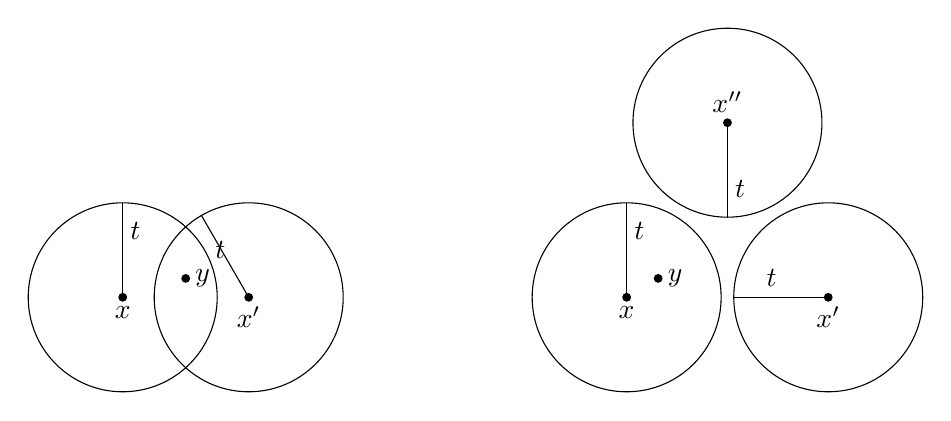
\begin{tikzpicture}[scale=0.8]
  \def\r{1.5}
  \def\eps{0.2}

  % left: overlapping spheres
  \begin{scope}[shift={(-5,0)}]
    \coordinate (A) at (0,0);
    \coordinate (B) at (2,0);

    \draw (A) circle (\r);
    \draw (B) circle (\r);

    \fill (A) circle (2pt);
    \fill (B) circle (2pt);

    \node[below] at (A) {$x$};
    \node[below] at (B) {$x'$};

    \draw (A) -- ($(A)+(0,\r)$);
    \node at ($(A)+(0.2,0.7*\r)$) {$t$};

    \draw (B) -- ($(B)+(-0.5*\r,0.866*\r)$);
    \node at ($(B)+(-0.3*\r,0.5*\r)$) {$t$};

    % point y
    \fill (1,0.3) circle (2pt);
    \node[right] at (1,0.3) {$y$};
  \end{scope}


  % right: disjoint spheres
  \begin{scope}[shift={(3,0)}]
    \coordinate (C) at (0,0);
    \coordinate (D) at ({2*\r+\eps},0);
    \coordinate (E) at ({(\r+\eps/2)}, {sqrt(3)*(\r+\eps/2)});

    \draw (C) circle (\r);
    \draw (D) circle (\r);
    \draw (E) circle (\r);

    \fill (C) circle (2pt);
    \fill (D) circle (2pt);
    \fill (E) circle (2pt);

    \node[below] at (C) {$x$};
    \node[below] at (D) {$x'$};
    \node[above] at (E) {$x''$};

    \draw (C) -- ($(C)+(0,\r)$);
    \node at ($(C)+(0.2,0.7*\r)$) {$t$};

    \draw (D) -- ($(D)+(-\r,0)$);
    \node at ($(D)+(-0.6*\r,0.3)$) {$t$};

    \draw (E) -- ($(E)+(0,-\r)$);
    \node at ($(E)+(0.2,-0.7*\r)$) {$t$};

    % point y
    \fill (0.5,0.3) circle (2pt);
    \node[right] at (0.5,0.3) {$y$};
  \end{scope}

\end{tikzpicture}
\end{center}

\end{thm}


\begin{defn}{}[Perfect codes]
  A code which achieves the sphere-packing bound is called a \emph{perfect code}.
  Thus, for a perfect $t$-error-correcting code, the $M$ spheres of radius $t$
  centred on codewords ‘fill’ the whole space $F_q^n$ without overlapping.

  In other words, every vector in $F_q^n$ is at distance $\leq t$ from exactly one codeword.
\end{defn}

\vspace{1.0cm}

\begin{thm}{}[MLCT problem (Version 1)]
  For given length $n$, find the maximum dimension $k$ such that $\exists$ an $[n, k, d]$-code over $GF(q)$. (Then, for this $k, B_q(n, d) = q^k)$.
\end{thm}

\begin{remark}{}
  \emph{redundancy} $r$ of an $[n, k, d]$-code is just $r=n-k$ (the number of check symbols in a codeword).
\end{remark}

\begin{thm}{}[MLCT problem (Version 2)]
  For given redundancy $r$, find the maximum length $n$ such that $\exists$ an $[n, n-r, d]$-code over $GF(q)$.
\end{thm}


\begin{defn}{}[$(n,s)$-set]
  a $(n, s)$-set in $V(r,q)$ is a set of $n$ vectors in $V(r, q)$ with the property that any $s$ of them are linearly independent.

  Denote $max_s(r,q)$ the largest value of $n$ for which $\exists$ a $(n,s)$-set
  in $V(r,q)$.\\
  ie.
  \begin{itemize}
    \item $(n,s)$-set: $n$ vectors with $s$ of them lin. independent
    \item $max_s(r,q)$: max $n$ for which $\exists~ (n,s)$-set
  \end{itemize}
\end{defn}

\begin{defn}{}[Packing problem]
  The \emph{packing problem} for $V(r,q)$ is that of determining the values of $max_s(r, q)$ and the optimal $(n,s)$-sets.
\end{defn}

\begin{thm}{14.1} \label{14.1}
There exists an $[n,n-r,d]$-code over $GF(q)$ iff $\exists$ an $(n, d-1)$-set in $V(r, q)$.
\end{thm}
\begin{proof}
  let $C$ a $[n, n-r, d]$-code over $GF(q)$ with PCM $H$. Then by Theorem \ref{8.4}, the columns of $H$ form a $(n, d-1)$-set in $V(r, q)$.

  On the other hand, let $K$ a $(n, d-1)$-set in $V(r, q)$. If we form a $r \times n$ matrix $H$ with the vectors of $K$ as its columns, by Theorem \ref{8.4}, $H$ is the PCM of a $[n, n-r]$-code whose minimum distance is at least $d$.
\end{proof}

\begin{cor}{14.2}
  for given values $q, d, r$, the largest value of $n$ for which there exists a $[n, n-r, d]$-code over $GF(q)$ is $max_{d-1}(r, q)$.
\end{cor}

$\Longrightarrow$ the MLCT problem (V2) is the same as the packing problem of finding $max_{d-1}(r, q)$.

\subsection{The projective geometry PG(r-1,q)}
Let the vector space
$$V(r,q)= \{ (a_1, a_2, \ldots, a_r) ~|~ a_i \in GF(q) \}$$

\begin{defn}{}[Projective Geometry]
  $PG(r-1, q)$
  \begin{itemize}
    \item \emph{points} are the one-dimensional subspaces of $V(r, q)$
    \item \emph{lines} are the two-dimensional subspaces of $V(r, q)$
  \end{itemize}

  Each point $P \in PG(r-1, q)$, as a subspace of $V(r,q)$ of dimension $1$, is generated by a single non-zero vector.

  So if $a=(a_1, a_2, \ldots, a_r) \in P$, then $P= \{ \lambda a ~|~ \lambda \in GF(q) \}$.

  $\Longrightarrow$ for $a=(a_1, a_2, \ldots, a_r),~b=(b_1, b_2, \ldots, b_r) \in P$, then
  $$a=b ~\text{in}~ PG(r-1,q) ~\text{iff}~ a=\lambda b ~\text{in}~ V(r,q)$$
  for some non-zero scalar $\lambda$.
\end{defn}

\begin{lemma}{14.6}
  in $PG(r-1,q)$,
  \begin{enumerate}
    \item number of points is $\frac{q^r-1}{q-1}$
    \item any two points lie on exactly one line
    \item each line contains exactly $q+1$ points
    \item each point lies on $\frac{q^{r-1} -1}{q-1}$ lines
  \end{enumerate}
\end{lemma}
\begin{proof}
  \begin{enumerate}
    \item number of points is $\frac{q^r-1}{q-1}$:\\
      since each of the $q^r-1$ nonzero vectors in $V(r,q)$ has $q-1$ nonzero scalar multiples, the number of points of $PG(r-1,q)$ is $\frac{q^r-1}{q-1}$

    \item any two points lie on exactly one line:\\
      if $a,b$ distinct points of $PG(r-1,q)$, then the unique line through them consists of the points $\lambda a + \mu b$, where $\lambda,\mu$ are scalars not both zero.

    \item each line contains exactly $q+1$ points:\\
      in (ii) there are $q^2-1$ choices for the pair $(\lambda, \mu)$, but we're identifying scalar multiples, so the number of distinct points on the line is
      $$\frac{q^2 -1}{q-1}=q+1$$

    \item each point lies on $\frac{q^{r-1} -1}{q-1}$ lines:\\
      let $t$ be the number of lines on which a point $P$ lies. Let the set
      $$X=\{(Q,L) ~|~ Q ~\text{is a point}~ \neq P,~ L~\text{is a line containing both}~ P ~\text{and}~ Q \}$$

      Count the members of $X$ in two ways:

      for each of the $\frac{q^r -1}{q-1} -1$ choices of $Q$, $\exists !$ line containing $P$ and $Q$. Thus,
      $$|X|=\frac{q^r-1}{q-1} -1 = \frac{q^r-q}{q-1}$$

      On the other hand, for each of the $t$ lines through $P$, there are (by (iii)) $q$ points $Q$ other than $P$ lying on $L$.

      Thus, $|X|=tq$,
      $$\Longrightarrow tq = \frac{q^r-q}{q-1}, ~~~~ \Longrightarrow t=\frac{q^{r-1}-1}{q-1}$$
  \end{enumerate}
\end{proof}

\begin{defn}{}[Projective plane]
  The $PG(2,q)$ is called the \emph{projective plane} over $GF(q)$.
\end{defn}

\section{MDS Codes}

\begin{thm}{15.1}
  a $[n, n-r, d]$-code satisfies $d \leq r+1$.
\end{thm}
\begin{proof}
  let $C$ a $[n, n-r, d]$-code, let $G=[ I_{n-r} ~|~ A]$ be a standard form GM of $C$.

  Since $A$ has $r$ columns, the codewords whicch are rows of $G$ have weight $\leq r+1$, ie. $w(C) \leq r+1$.

  The result follows from Theorem \ref{5.2},
  \begin{align*}
  &\Longrightarrow~ w(C)=d(C)\\
  &\Longrightarrow~ d(C) \leq r+1.
  \end{align*}
\end{proof}

\begin{defn}{}[MDS]
  a $[n, n-r, r+1]$-code,\\
  \hspace*{2em}ie. a linear cocde of redundancy $r$ whose min. distance is $r+1$,\\
  is called a \emph{maximum distance separable code}, MDS.

  $\longrightarrow$ by Theorem \ref{14.1}, max length of a MDS code over $GF(q)$ is $max_r(r,q)$, the largest size of a $(n,r)$-set in $V(r,q)$.
\end{defn}

\begin{conj}{15.2}
  if $2 \leq r \leq q$, then $max_r(r,q)=q+1$

  (except $max_3(3,q)=max_{q-1}(q-1,q)=q+2$ if $q=2^h$)
\end{conj}

\begin{thm}{15.3}
  if $r\geq q$, then $max_r(r,q)=r+1$. Any MDS code of redundancy $r\geq q$ is equivalent to a repetition code of length $r+1$.
\end{thm}
\begin{proof}
  repetition code of length $r+1$: a $[r+1, 1, r+1]$-code with GM $[1~1~\cdots~1]$.

  Hence $max_r(r,q) \geq r+1$.

  Also, any $[r+1, 1, r+1]$-code is equivalent to a repetition code.

  Suppose $r \geq q$ and by contradiction that $max_r(r,q) \geq r+2$.

  Then, $\exists$ a $[r+2, 2, r+1]$-code $C$ over $GF(q)$.

  $\longrightarrow~C$ must be equivalent to a code having GM:
  $$G=
  \begin{bmatrix}
    1 & 0 & 1 & 1 & \ldots & 1\\
    0 & 1 & a_1 & a_2 & \ldots & a_r
  \end{bmatrix}
  $$

  in order that any linear combination of the rows of $G$ has weight at least $r+1$ with $0 \neq a_i \in GF(q)$.

  This implies $r \leq q-1$, contradiction.
\end{proof}

\begin{remark}{}
  the only binary MDS codes are\\
  $V(n,2)$, the even weighted codes $E_n$, and repetition codes.
\end{remark}

\begin{thm}{15.4}
  let $2 \leq r \leq q$, let $a_1, a_2, \ldots, a_{q-1} \in GF(q)$ nonzero.

  Then,
  $$
  H =
  \begin{bmatrix}
    1 & 1 & \ldots & 1 & 1 & 0\\
    a_1 & a_2 & \ldots & a_{q-1} & 1 & 0\\
    a_1^2 & a_2^2 & \ldots & a_{q-1}^2 & 1 & 0\\
     & & & & \vdots & \vdots\\
    \vdots & \vdots & & \vdots & 0 & 0\\
    a_1^{r-1} & a_2^{r-1} & \ldots & a_{q-1}^{r-1} & 0 & 1
  \end{bmatrix}
  $$

  is the PCM of a MDS $[q+1, q+1-r, r+1]$-code.

  Equivalently, the columns of $H$ form a $(q+1)$-arc in $PG(r-1, q)$.
\end{thm}
\begin{proof}
  the determinant of a matrix formed by any $r$ columns of $H$ is equal to the determinant of a Vandermonde matrix, and so is non-zero (see a proof of this at section \ref{sec:vandermondedet}).
  Thus any $r$ columns of $H$ are linearly independent.
\end{proof}

\begin{cor}{15.7}
  The dual code of a MDS code is also MDS.
\end{cor}
\begin{cor}{15.8}
  $\exists$ a MDS $[n,k]$-code over $GF(q)$ iff $\exists$ a MDS $[n, n-k]$-code over $GF(q)$.
\end{cor}


\subsection{Vandermonde determinant} \label{sec:vandermondedet}

This section contains a simple proof of the Vandermonde matrix determinant. The proof was found in \cite{vanddetproof}, here it is written with small modifications and expanded. A different proof can be found in \cite{vanddetproof2}.

\begin{lemma}{}[Vandermonde determinant]
$$
\det~V(x_1, ..., x_n) = \det
\begin{pmatrix}
    1 & x_1 & x_1^2 & \ldots & x_1^{n-1} \\
    1 & x_2 & x_2^2 & \ldots & x_2^{n-1} \\
    1 & x_3 & x_3^2 & \ldots & x_3^{n-1} \\
    \vdots & \vdots & \vdots &  & \vdots\\
    1 & x_n & x_n^2 & \ldots & x_n^{n-1} \\
\end{pmatrix}
= \prod_{j < i} (x_i - x_j)
$$
\end{lemma}

\begin{proof}

The equation is true for $n = 2$, as we have:

$$
\det~V(x_1, x_2) = \det
\begin{pmatrix}
    1 & x_1\\
    1 & x_2
\end{pmatrix}
= x_2 - x_1
$$

We now assume that $n \ge 3$. Starting with column $n$ and ending at column $2$, we successively apply the following operation: subtract $x_1$ times column $i-1$ from column $i$. The determinant remains the same and the resulting matrix is:

$$
= \det
\begin{pmatrix}
    1 & x_1-(x_1 \cdot 1) & x_1^2 - (x_1 \cdot x_1) & \ldots & x_1^{n-1} - (x_1 \cdot x_1^{n-2}) \\
    1 & x_2-(x_1 \cdot 1) & x_2^2 - (x_1 \cdot x_2) & \ldots & x_2^{n-1} - (x_1 \cdot x_2^{n-2}) \\
    1 & x_3-(x_1 \cdot 1) & x_3^2 - (x_1 \cdot x_3) & \ldots & x_3^{n-1} - (x_1 \cdot x_3^{n-2}) \\
    \vdots & \vdots & \vdots &  & \vdots\\
    1 & x_n-(x_1 \cdot 1) & x_n^2 - (x_1 \cdot x_n) & \ldots & x_n^{n-1} - (x_1 \cdot x_n^{n-2}) \\
\end{pmatrix}
$$
$$
= \det
\begin{pmatrix}
    1      & 0           & 0              & \ldots & 0 \\
    1      & (x_2 - x_1) & x_2(x_2 - x_1) & \ldots & x_2^{n-2}(x_2 - x_1) \\
    1      & (x_3 - x_1) & x_3(x_3 - x_1) & \ldots & x_3^{n-2}(x_3 - x_1) \\
    \vdots & \vdots      & \vdots         &        & \vdots \\
    1      & (x_n - x_1) & x_n(x_n - x_1) & \ldots & x_n^{n-2}(x_n - x_1) \\
\end{pmatrix}
$$

Applying the Laplace expansion along the first row and factoring out the scalar multiples $(x_i - x_1)$ in each column, we obtain: 

$$
= \det
\begin{pmatrix}
    x_2-x_1 & x_2^2 - x_1 x_2 & x_2^3 - x_1 x_2^2 & \ldots & x_2^{n-1} - x_1 x_2^{n-2} \\
    x_3-x_1 & x_3^2 - x_1 x_3 & x_3^3 - x_1 x_3^2 & \ldots & x_3^{n-1} - x_1 x_3^{n-2} \\
    \vdots & \vdots & \vdots &  & \vdots\\
    x_n-x_1 & x_n^2 - x_1 x_n & x_n^3 - x_1 x_n^2 & \ldots & x_n^{n-1} - x_1 x_n^{n-2} \\
\end{pmatrix}
$$

in each row, factor out $(x_i - x_1)$

$$
= \det
\begin{pmatrix}
    1(x_2-x_1) & x_2(x_2 - x_1) & x_2^2(x_2 - x_1) & \ldots & x_2^{n-2}(x_2 - x_1) \\
    1(x_3-x_1) & x_3(x_3 - x_1) & x_3^2(x_3 - x_1) & \ldots & x_3^{n-2}(x_3 - x_1) \\
    \vdots & \vdots & \vdots &  & \vdots\\
    1(x_n-x_1) & x_n(x_n - x_1) & x_n^2(x_n - x_1) & \ldots & x_n^{n-2}(x_n - x_1) \\
\end{pmatrix}
$$
$$
= \prod_{2 \leq i \leq n} (x_i - x_1) ~~\det
\begin{pmatrix}
    1 & x_2 & x_2^2 & \ldots & x_2^{n-2} \\
    1 & x_3 & x_3^2 & \ldots & x_3^{n-2} \\
    \vdots & \vdots & \vdots &  & \vdots\\
    1 & x_n & x_n^2 & \ldots & x_n^{n-2} \\
\end{pmatrix}
$$

now, by induction

$$
= \prod_{i=2}^n (x_i - x_1) ~~\cdot \prod_{2 \leq j < i \leq n} (x_i - x_j) ~~= \prod_{1 \leq j < i \leq n} (x_i - x_j)
$$
\end{proof}


\vspace{1.0cm}

\section{Cyclic Codes}

\subsection{Cyclic Codes intro}

\begin{defn}{}{cyclic code}
  a code $C$ is cyclic if
  \begin{enumerate}[i.]
    \item $C$ is a linear code
    \item any cyclic shift of a codeword is also a codeword\\
      ie. when $a_0 a_1 \ldots a_{n-1} \in C$,\\
      then so $a_{n-1} a_0 a_1 \ldots a_{n-2} \in C$.
  \end{enumerate}
\end{defn}

\begin{remark}{}[Notation]
  From now on,
  $$F = F_q = \mathbb{F} = GF(q)$$

  $F_q[x]$ is a ring; and for $f(x)$ irreducible in $F_q[x]$, then $\frac{F_q[x]}{f(x)}$ is a field.

  From now on,
$$f(x) = x^n -1 ~~~\Longrightarrow~~ F_q[x]/(x^n-1) = R_n$$

  \vspace{0.6cm}
  Observe:\\
  since $x^n \cong 1 \bmod{x^n -1}$, to reduce any polynomial by modulo $x^n-1$ can just replace $x^n$ by $1$, $x^{n+1}$ by $x$, $x^{n+2}$ by $x^2$, etc.

  \vspace{0.6cm}
  Correspondence:
  $$a_0 a_1 \ldots a_{n-1} \in V(n,q) ~\Longleftrightarrow~ a(x)=a_0 + a_1 x + \ldots + a_{n-1} x^{n-1} \in R_n$$

  In $R_n$,
  \begin{align*}
    x \cdot a(x) &= a_0 \cdot x + a_1 x^2 + \ldots + \underbrace{a_{n-1} x^n}_{=a_{n-1}\cdot 1}\\
                 &=a_{n-1} + a_0 x + \ldots + a_{n-2} \cdot x^{n-1} \in R_n
  \end{align*}

  ie. $a_{n-1} a_0 a_1 \ldots a_{n-2} \in V(n, q)$

  \vspace{0.6cm}
  In $R_n$:
  \begin{itemize}
    \item[$\rightarrow$] multiply by $x$ corresponds to performing a single cyclic shift
    \item[$\rightarrow$] multiply by $x^m$ corresponds to a cyclcic shift through $m$ positions
  \end{itemize}
\end{remark}


\vspace{1.0cm}
\begin{thm}{12.6}[Algebraic characterization of cyclic codes] \label{12.6}
  a code $C \in R_n$ is a cyclic code iff
  \begin{enumerate}[i.]
    \item $a(x),b(x) \in C ~\Longrightarrow~ a(x)+b(x) \in C$
    \item $a(x) \in C$ and $r(x) \in R_n ~\Longrightarrow~ r(x) a(x) \in C$\\
      ie. $C$ closed under multiplication by any element of $R_n$
  \end{enumerate}
\end{thm}
\begin{proof}
  \begin{enumerate}[i.]
    \item let $C \in R_n$ cyclic code, then $C$ is linear, so (i) holds.
    \item let $a(x) \in C$ and $r(x) = r_0 + r_1 x + \ldots + r_{n-1} x^{n-1} \in R_n$.

      Since mult. by $x$ corresponds to a cyclic shift, then $x \cdot a(x) \in C$, thus
      $$x \cdot (x \cdot a(x)) = x^2 \cdot a(x) \in C$$
      and so on.

      Hence,
      $$r(x) \cdot a(x) = r_0 \cdot a(x) + r_1 \cdot x \cdot a(x) + \ldots + r_{n-1} \cdot x^{n-1} \cdot a(x) \in C$$
      since each summand is in $C$; thus (ii) holds.

      \vspace{0.5cm}
      Conversely, suppose (i) and (ii) hold;\\
      taking $r(x)$ to be a scalar, the conditions imply that $C$ is linear.\\
      Taking $r(x)=x$, in (ii) shows that $C$ is cyclic.
  \end{enumerate}
\end{proof}

\begin{remark}{}
  \begin{enumerate}[i.]
    \item Cyclic codes are the ideals of the ring $R_n$.
    \item Every ideal in $R_n$ is a \emph{principal ideal}.\\
      ie. $R_n$ is a PID.
  \end{enumerate}
\end{remark}

\vspace{1.0cm}
Let $f(x) \in R_n$, $\langle f(x) \rangle$ the subset of $R_n$ consisting of all multiples of $f(x)$ (reduced modulo $x^n-1$). ie.
$$\langle f(x) \rangle = \{ r(x) \cdot f(x) ~|~ r(x) \in R_n \}$$


\begin{thm}{12.7}
  for any $f(x) \in R_n$, the set $\langle f(x) \rangle$ is a cyclic code; named the \emph{code generated by $f(x)$}.
\end{thm}
\begin{proof}
  check conditions (i), (ii) of Theorem \ref{12.6}:
  \begin{enumerate}[i.]
    \item if $a(x)f(x),~ b(x)f(x) \in \langle f(x) \rangle$ then
      $$a(x)f(x)+b(x)f(x)= (a(x)+ b(x)) f(x) \in \langle f(x) \rangle$$

    \item if $a(x)f(x) \in \langle f(x) \rangle$ and $r(x) \in R_n$, then
      $$r(x) (a(x)f(x))= (r(x) \cdot a(x)) f(x) \in \langle f(x) \rangle$$
  \end{enumerate}
\end{proof}

\begin{eg}{12.8}
  $C=\langle 1+x^2 \rangle \in R_3$, with $GF(2)$.

  $R_3$ has $2^3=8$ elements.

  Multiply $1+x^2$ by each of the 8 elements of $R_3$ (reducing modulo $x^3-1$), obtaining 4 distinct codewords:
  $$0, 1+x, 1+x^2, x+x^2$$
  Thus $C$ is the code $\{ 000, 110, 101, 011 \}$.
\end{eg}


\begin{thm}{12.9} \label{12.9}
  let $C$ a nonzero cyclic coded in $R_n$. Then
  \begin{enumerate}[i.]
    \item $\exists !~ g(x)$ monic, of smallest degree in $C$
    \item $C=\langle g(x) \rangle$
    \item $g(x)$ is a factor of $x^n -1$
  \end{enumerate}
\end{thm}
\begin{proof}
  \begin{enumerate}[i.]
    \item $\exists !~ g(x)$ monic, of smallest degree in $C$:\\
      let $g(x), h(x) \in C$ monic and of smallest degree. Then $g(x)-h(x) \in C$ with smaller degree, which is a contradiction if $g(x) \neq h(x)$

    \item $C=<g(x)>$:\\
      let $a(x) \in C$. By division algorithm for $F_q[x]$,
      $$a(x) = q(x) g(x) + r(x)$$
      with $deg(r(x)) < deg(g(x))$.

      But $r(x) = a(x) - q(x)g(x) \in C$ by the properties of cyclic codes (Theorem \ref{12.6}, $a,g \in C$ and $C$ an ideal)

      By minimality of $deg(g(x))$, must have $r(x) = 0$, therefore
      $$a(x) \in \langle g(x) \rangle \forall a(x) \in C$$
      $$\Longrightarrow~ C=\langle g(x) \rangle$$

    \item $g(x)$ is a factor of $x^n -1$:\\
      by division algorithm,
      $$x^n -1 = q(x) g(x) + r(x)$$
      with $deg(r(x)) < deg(g(x))$.

      But then $r(x) = -q(x) g(x) \bmod{x^n -1}$, ie. $r(x)$ is a multiple of $g(x)$, and so $r(x) \in \langle g(X) \rangle$.

      By the minimality of $deg(g(x))$, we must have $r(X)=0$, which implies
      $$x^n -1 = q(x) \cdot g(x) + 0$$
      $\Longrightarrow~ g(x)$ is a factor of $(x^n-1)$.
  \end{enumerate}
\end{proof}


\begin{defn}{}[Generator polynomial]
  let $C$ cyclic code, monic polynomial of least ddegree (given by Theorem \ref{12.9}) is called the \emph{generator polynomial} of $C$.

  Note: $C$ may contain other polynomials than the generator polynomial which also generate $C$.
\end{defn}

\subsection{Recap on ideals}
More about ideals at the \emph{Commutative Algebra notes} \cite{commutativealgebranotes}.
\vspace{0.6cm}

In the cyclic codes context, we're interested in ideals because
\begin{itemize}
  \item cyclic codes are ideals of $R_n = \mathbb{F}_q[x]/(x^n-1)$.
  \item $R_n$ is a PID: every ideal in $R_n$ is principal.
\end{itemize}

\vspace{0.6cm}

\begin{defn}{}[ideal]
  $I \subset R$ ($R$ ring) such that $0 \in I$ and $\forall x \in I,~ r \in R,~ xr, rx \in I$.\\
  \hspace*{2em} ie. $I$ absorbs products in $R$.
\end{defn}

\begin{defn}{}[prime ideal]
  if $a, b \in R$ with $ab \in P$ and $P \neq R$ ($P$ a prime ideal), implies $a \in P$ or $b \in P$.
\end{defn}

\begin{defn}{}[principal ideal]
  generated by a single element, $(a)$.

  $(a)$: principal ideal, the set of all multiples $xa$ with $x \in R$.
\end{defn}

\begin{defn}{}[prime spectrum - $Spec(A)$]
  set of prime ideals of $A$. ie.

  $$Spec(A) = \{ P ~|~ P \subset A~ \text{is a prime ideal} \}$$
\end{defn}

\begin{defn}{}[integral domain]
  Ring in which the product of any two nonzero elements is nonzero.

  ie. no zerodivisors.

  ie. $\forall~ 0 \neq a,~ 0 \neq b \in A,~ ab \neq 0 \in A$.

  Every field is an integral domain, not the converse.
\end{defn}

\begin{defn}{}[principal ideal domain - PID]
  integral domain in which every ideal is principal. ie.
  ie. $\forall I \subset R,~ \exists~ a \in I$ such that $I = (a) = \{ ra ~|~ r \in R \}$.
\end{defn}



\bibliographystyle{unsrt}
\bibliography{algebraic-coding-theory-notes.bib}

\end{document}
